% (The MIT License)
%
% Copyright (c) 2023-2024 Yegor Bugayenko
%
% Permission is hereby granted, free of charge, to any person obtaining a copy
% of this software and associated documentation files (the 'Software'), to deal
% in the Software without restriction, including without limitation the rights
% to use, copy, modify, merge, publish, distribute, sublicense, and/or sell
% copies of the Software, and to permit persons to whom the Software is
% furnished to do so, subject to the following conditions:
%
% The above copyright notice and this permission notice shall be included in all
% copies or substantial portions of the Software.
%
% THE SOFTWARE IS PROVIDED 'AS IS', WITHOUT WARRANTY OF ANY KIND, EXPRESS OR
% IMPLIED, INCLUDING BUT NOT LIMITED TO THE WARRANTIES OF MERCHANTABILITY,
% FITNESS FOR A PARTICULAR PURPOSE AND NONINFRINGEMENT. IN NO EVENT SHALL THE
% AUTHORS OR COPYRIGHT HOLDERS BE LIABLE FOR ANY CLAIM, DAMAGES OR OTHER
% LIABILITY, WHETHER IN AN ACTION OF CONTRACT, TORT OR OTHERWISE, ARISING FROM,
% OUT OF OR IN CONNECTION WITH THE SOFTWARE OR THE USE OR OTHER DEALINGS IN THE
% SOFTWARE.

\documentclass{article}
\usepackage{../osbp}
\newcommand*\thetitle{Integrating}
\begin{document}

\plush{\lnTitlePage{6}{8}{iyJ4wiCb9xM}}

\lnThought{Setup continuous integration in order to prove that your product works}

\lnQuote
  [Bogdan Vasilescu]
  {bogdan-vasilescu}
  {Teams using CI are significantly more effective at merging pull requests submitted by core members. Availability of CI is also associated with external contributors having fewer pull requests rejected.}
  {vasilescu2015quality}

\lnQuote
  [Pei Liu]
  {pei-liu}
  {We start by collecting a set of 84,475 open-source Android apps from the most popular three online code hosting sites, namely Github, GitLab, and Bitbucket. We then look into those apps and find that only around 10\% of apps have leveraged CI/CD services, i.e., the \ul{majority} of open-source Android apps are developed \ul{without} accessing CI/CD services.}
  {liu2022first}

\lnQuote
  [Mehdi Golzadeh]
  {mehdi-golzadeh}
  {Together with Travis, GHA covers more than 80\% of all usages. Moreover, in only 18 months GHA has overtaken all other CIs in popularity.}
  {golzadeh2022rise}
\lnPitch{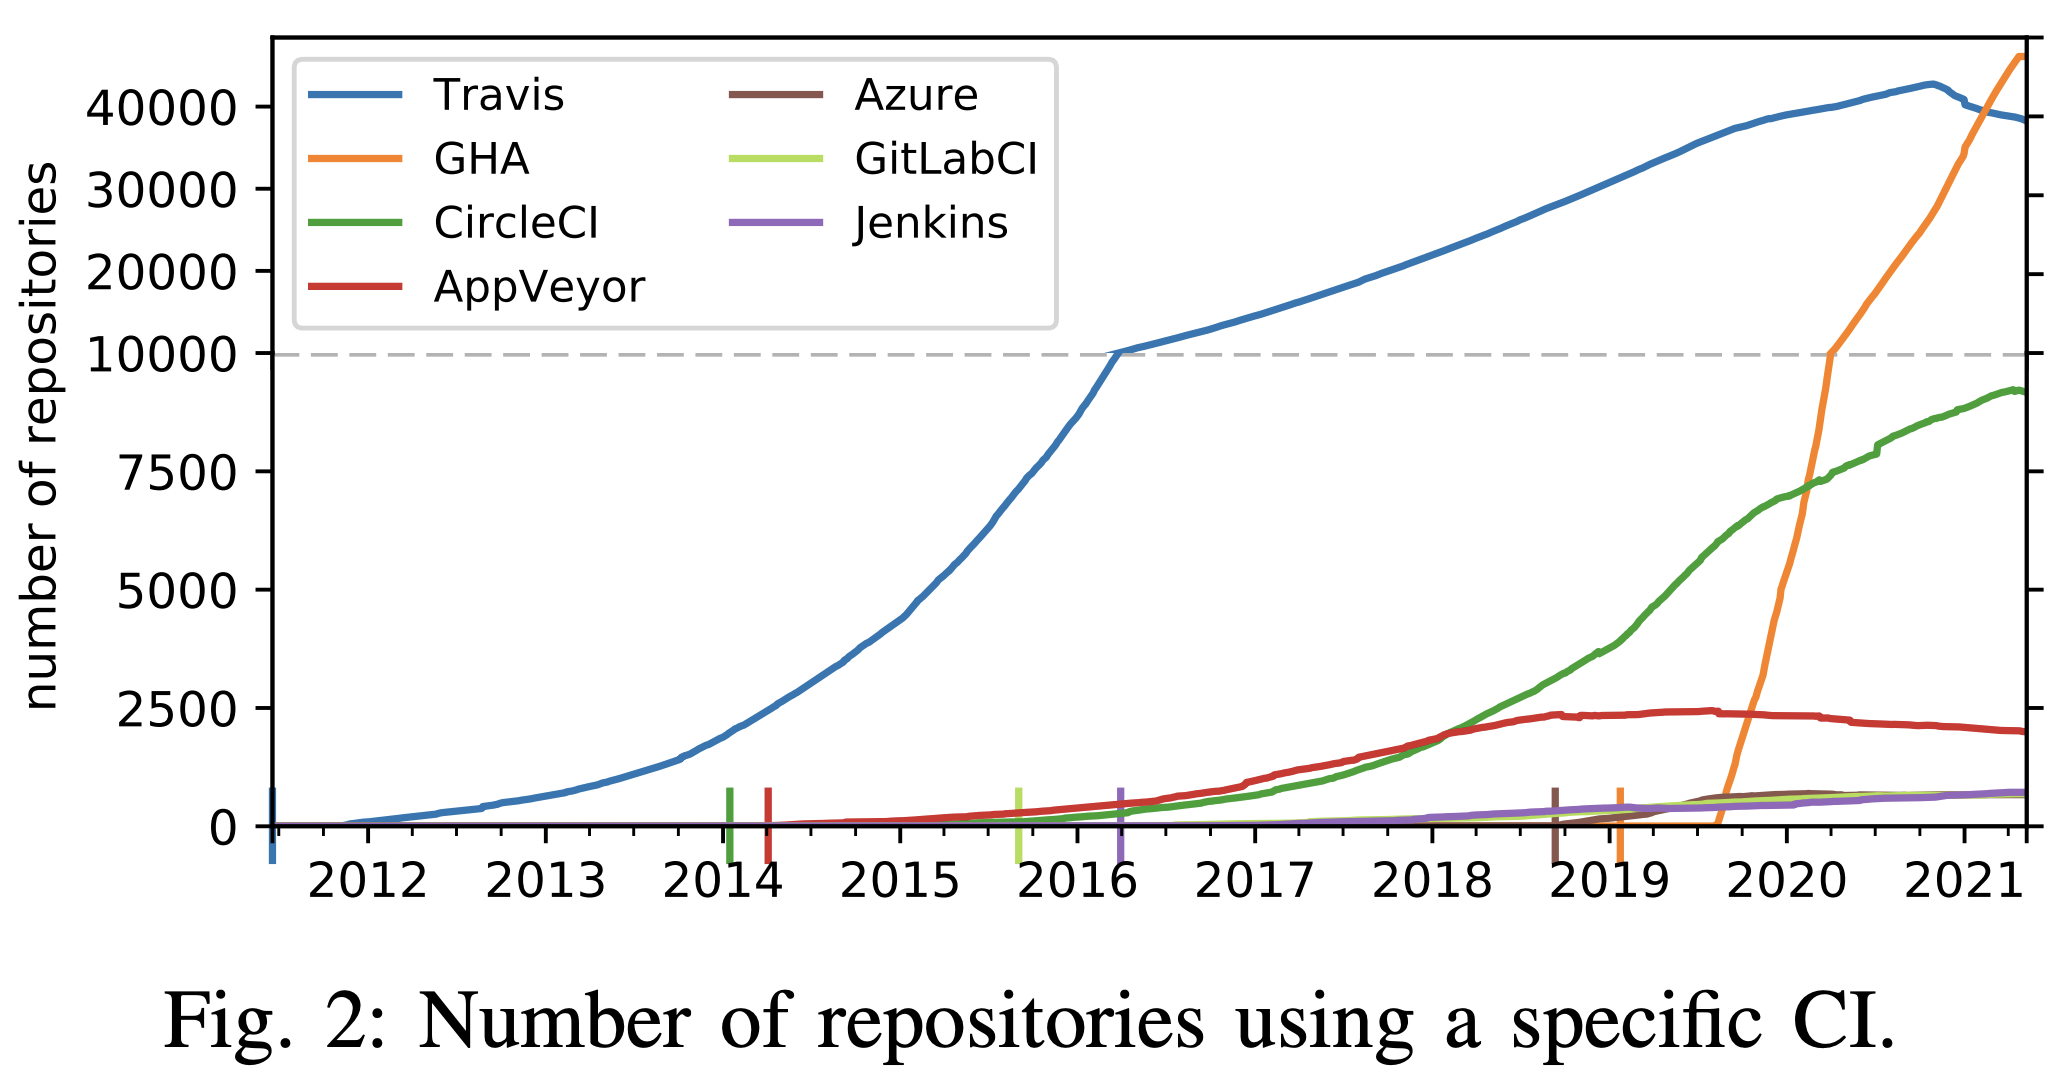
\includegraphics[width=.75\linewidth]{gha-growth.png}
  \lnSource{golzadeh2022rise}}

\lnThought{Use fixed versions of dependencies}

\lnThought{Use build matrix, with fixed versions}

\lnPitch{
  \begin{multicols}{2}
  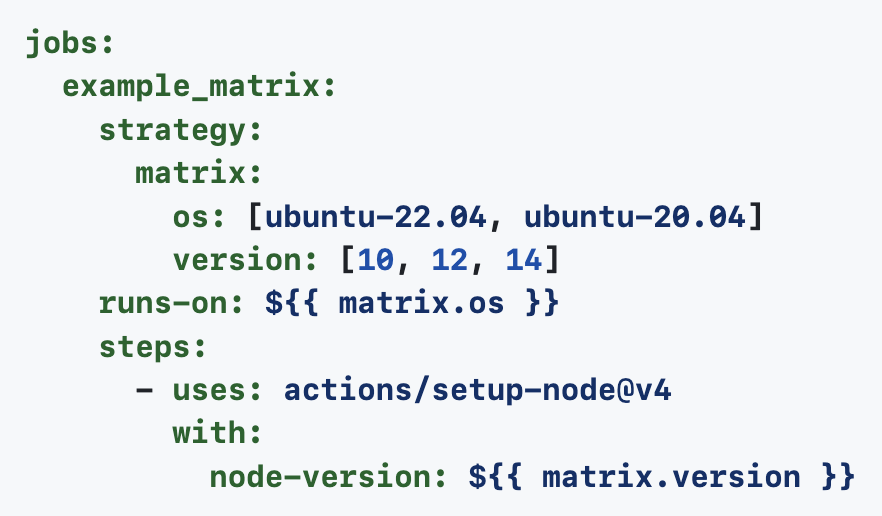
\includegraphics[width=.9\linewidth]{matrix.png}
  \par\columnbreak\par
  ``A matrix strategy lets you use variables in a single job definition to automatically create multiple job runs that are based on the \ul{combinations} of the variables. For example, you can use a matrix strategy to test your code in multiple versions of a language or on multiple operating systems.''
  \par
  --- \href{https://docs.github.com/en/actions/using-jobs/using-a-matrix-for-your-jobs}{GitHub}
  \end{multicols}}

\lnQuote
  [Moritz Beller]
  {moritz-beller}
  {The use of multiple integration environments leads to 10\% \ul{more failures} being caught at build time.}
  {beller2017oops}

\lnPitch{
  \begin{multicols}{2}
  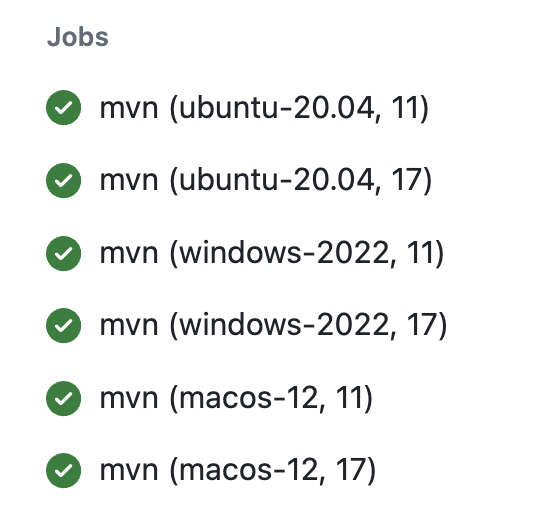
\includegraphics[width=.9\linewidth]{xembly-matrix.png}
  \par
  {\small GitHub Actions in \href{https://github.com/yegor256/xembly}{yegor256/xembly}\par}
  \par\columnbreak\par
  ``One might argue that it therefore only makes sense to do continuous integration in several environments when their execution leads to \ul{different results}, capturing errors that would not have been caught with one single environment.''
  \lnSource{beller2017oops}
  \end{multicols}}

\lnThought{Provide \ff{Dockerfile}}

\lnPitch{
  \begin{multicols}{2}
  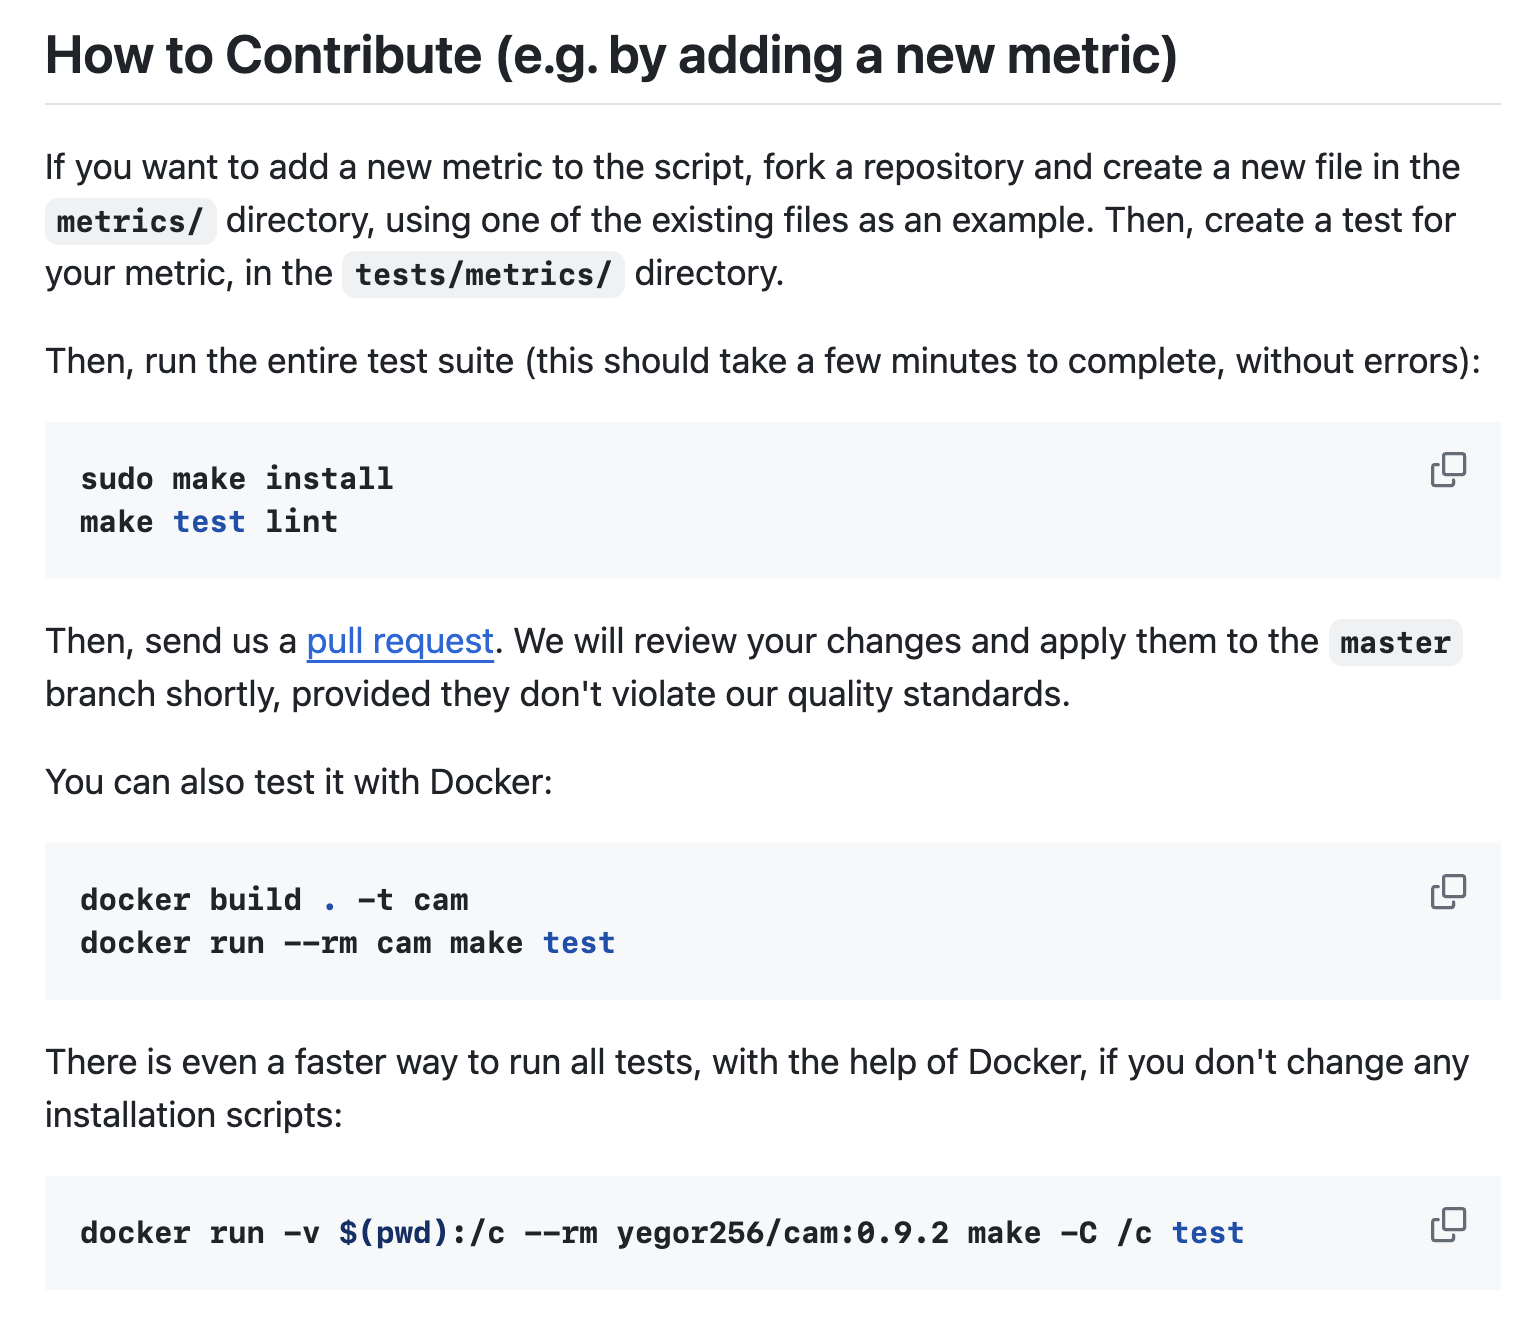
\includegraphics[width=.9\linewidth]{cam-how-to.png}
  \par
  {\small \url{https://github.com/yegor256/cam}\par}
  \par\columnbreak\par
  ``One of the largest benefits about Dockerfiles is that they can be completely \ul{self contained}. Your CI vendor of choice starts to matter less and less because the Dockerfiles themselves are portable and predictable.''
  \lnSource{batilo2022ways}
  \end{multicols}}

\lnThought{Be aware of flaky tests}

\lnQuote
  [Thomas Durieux]
  {thomas-durieux}
  {We observe that developers restart at least 1.72\% of builds, amounting to 56,522 restarted builds in our Travis CI dataset. We observe that more \ul{mature} and more \ul{complex} projects are more likely to include restarted builds. The restarted builds are mostly builds that are initially failing due to a \ul{test}, \ul{network problem}, or a Travis CI \ul{limitations} such as execution timeout.}
  {durieux2020empirical}

\lnThought{Enable @renovate or @dependabot}

\lnThought[bugayenko2023blog0822]{Discriminate tests as fast and slow}

\lnThought{Use caching in GitHub Action}

\lnQuote
  [Islem Bouzenia]
  {islem-bouzenia}
  {The majority of the used resources is consumed by testing and building (91.2\%), which is triggered by pull requests (50.7\%), pushes (30.9\%), and regularly scheduled workflows (15.5\%). While existing optimizations, such as \ul{caching} (adopted by 32.9\% of paid-tier repositories), demonstrate a positive impact, they overall remain \ul{underutilized}.}
  {bouzenia2024resource}

\lnThought{Implement your own GitHub Actions}

\lnQuote
  [Sk Golam Saroar]
  {sk-golam-saroar}
  {We found that developers find the composition of YAML files, which are essential for GitHub Action integration, \ul{challenging} and \ul{error-prone}.}
  {saroar2023developers}
\lnPitch{
  \begin{multicols}{2}
  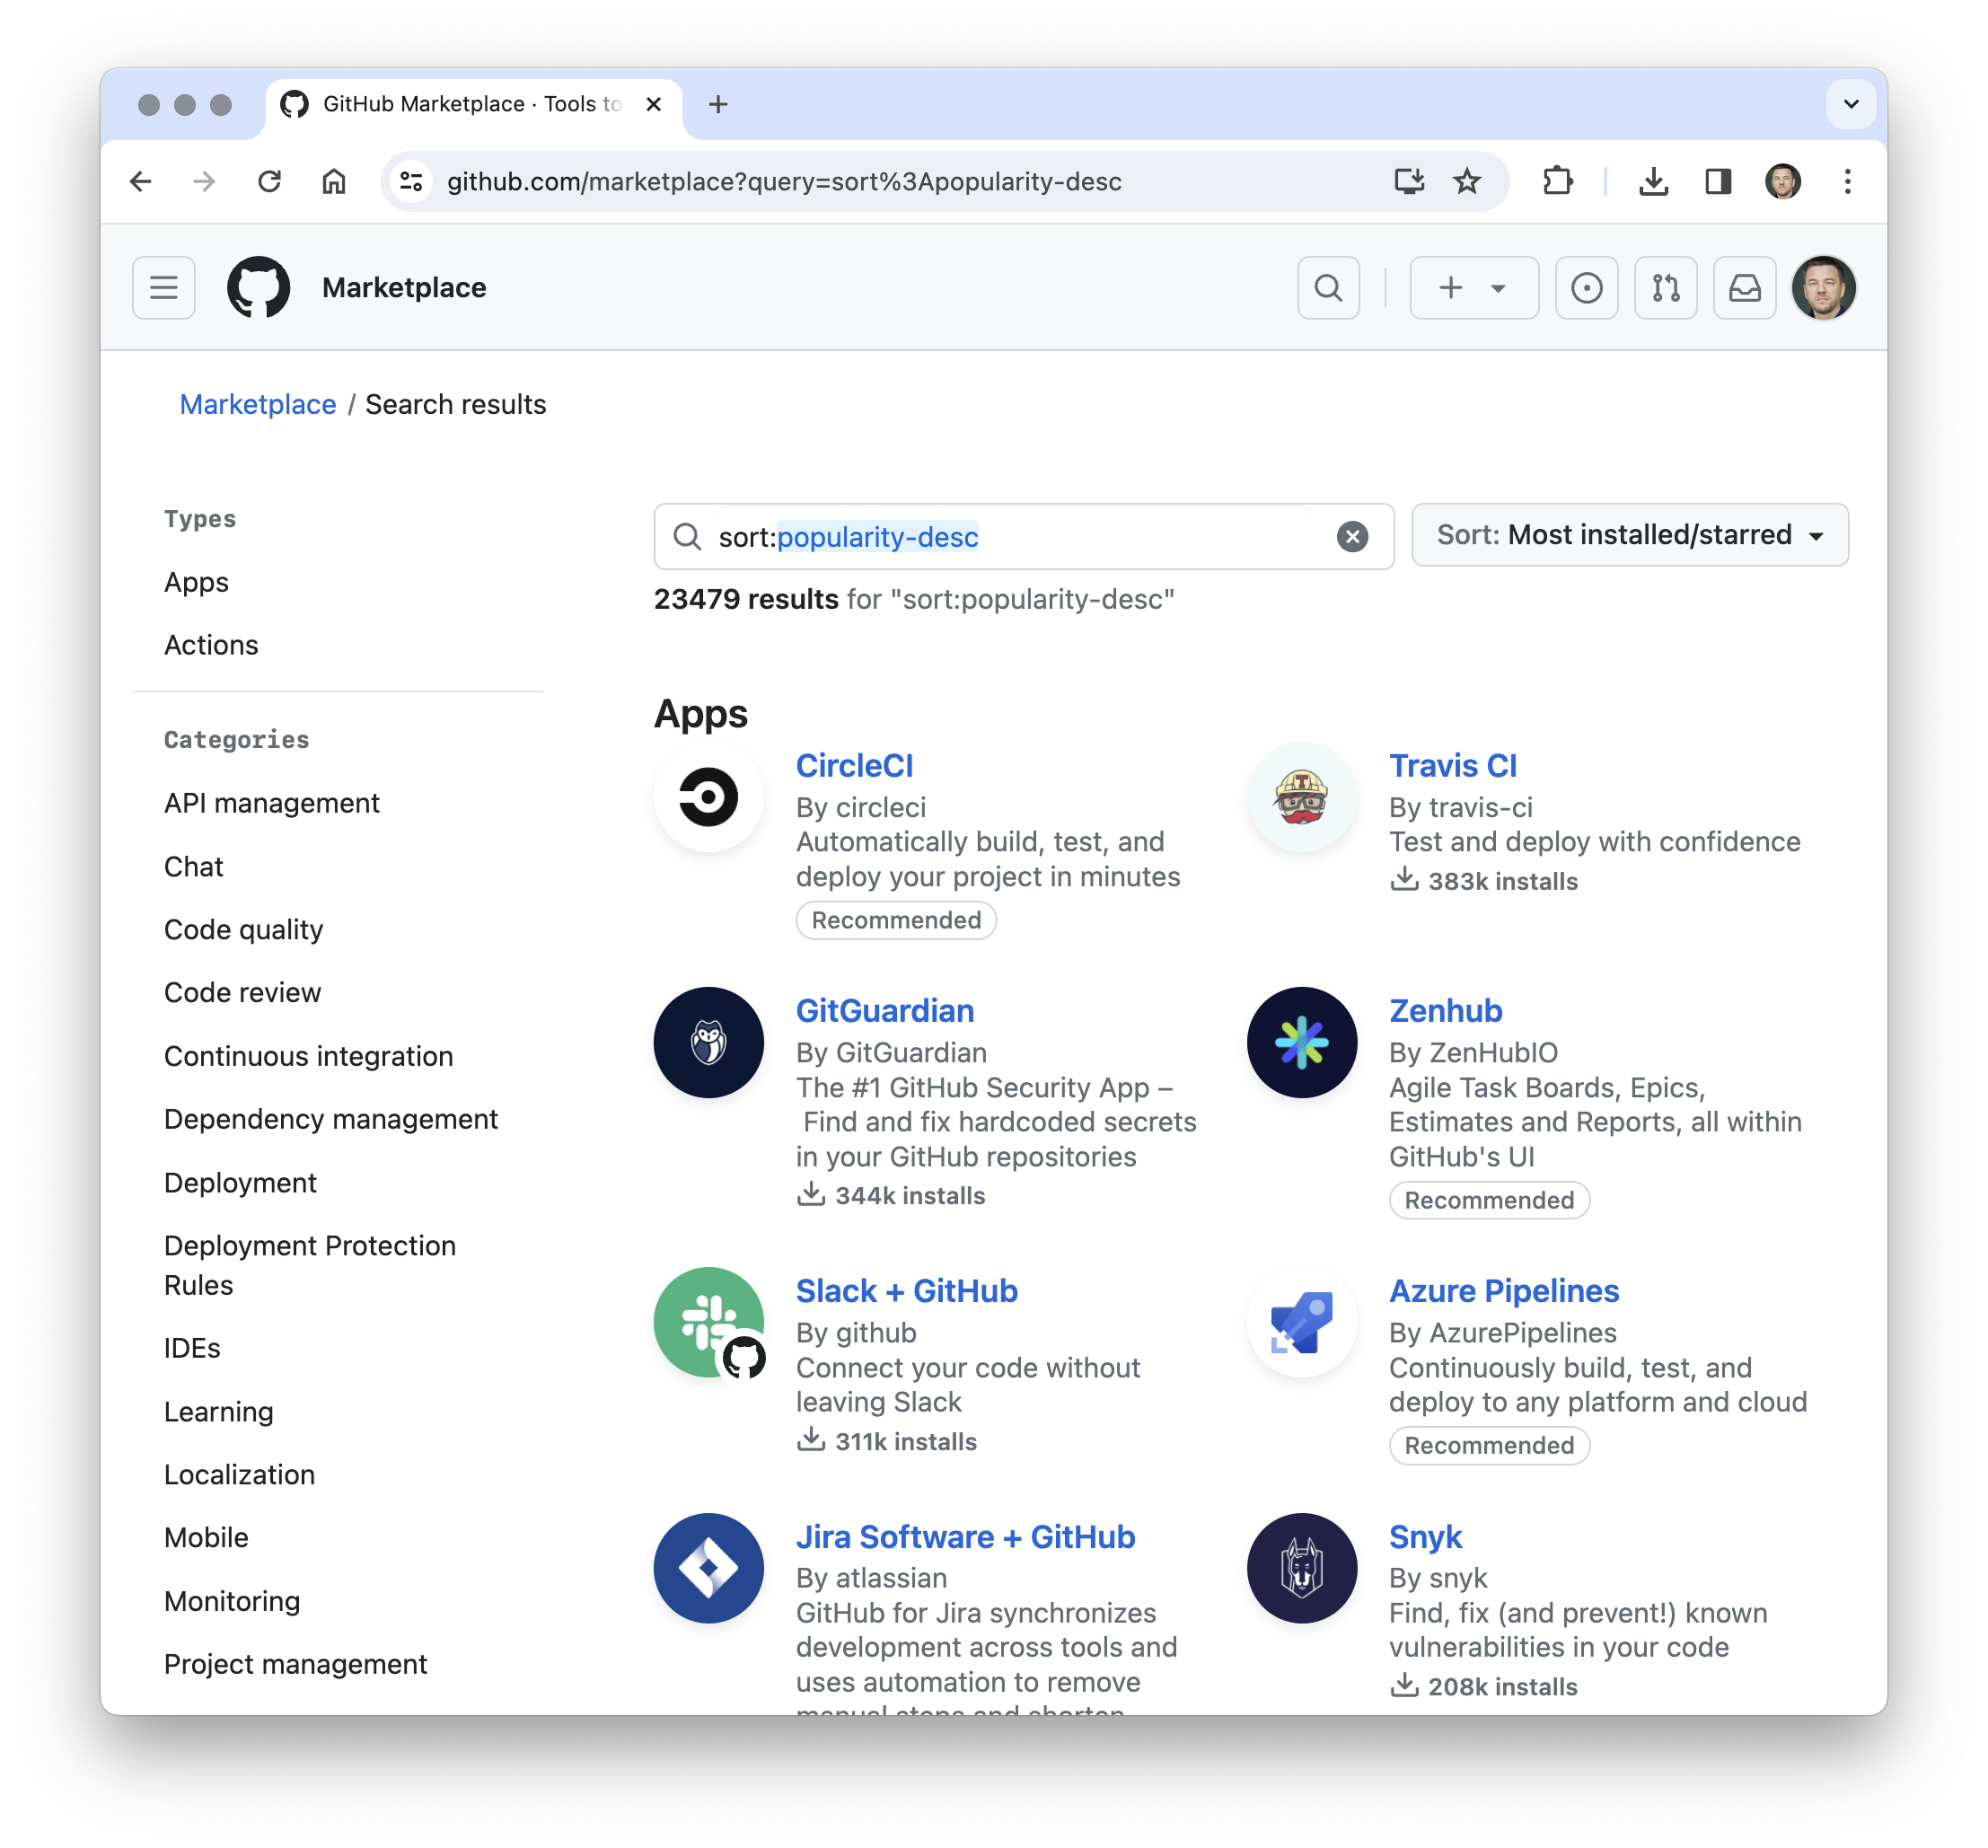
\includegraphics[width=.9\linewidth]{actions.png}
  \par
  {\small \url{https://github.com/marketplace}\par}
  \par\columnbreak\par
  ``While there are over \ul{15,000} Actions in existence, an increasing number of Actions are published every day on the Marketplace. This creates the question as to why developers prefer to develop new Actions rather than reusing the existing ones.''
  \lnSource{saroar2023developers}
  \end{multicols}}
\lnPitch{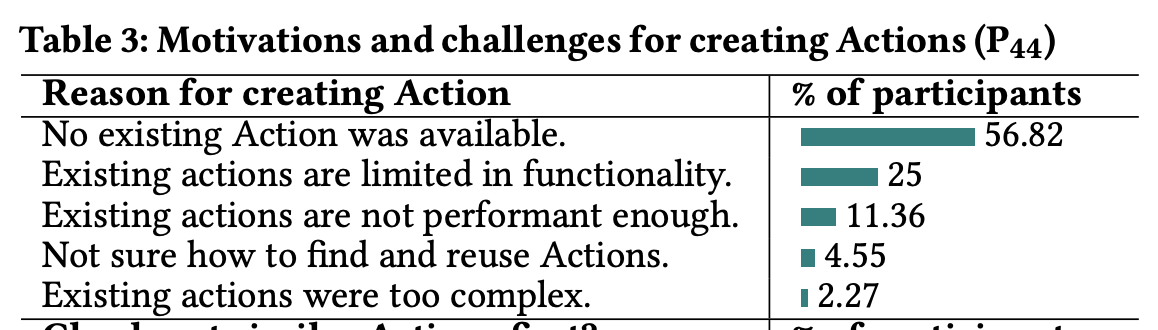
\includegraphics[width=.75\linewidth]{why-action.png}
  \lnSource{saroar2023developers}}

\end{document}
